%% This is an example first chapter.  You should put chapter/appendix that you
%% write into a separate file, and add a line \include{yourfilename} to
%% main.tex, where `yourfilename.tex' is the name of the chapter/appendix file.
%% You can process specific files by typing their names in at the 
%% \files=
%% prompt when you run the file main.tex through LaTeX.
\chapter{Introduction}\label{ch1:intro}
The pursuit of energy has shaped the history of mankind from the very beginning. And while the image of ancient humans huddled around fires for warmth, protection, and meal preparation is an archetype of our ancestral past, modern human needs remain much the same. Lighting to extend day into night, heating and cooling for residential comfort, cooking of the food we eat, access to the advanced technologies of our time – these all require energy from one source or another. Choices abound, from animal and plant-based fuels, to buried hydrocarbon resources, to alternatives like solar, wind, hydro, nuclear, and geothermal. The balance and utilization of these resources can shape societal growth on the geopolitical stage and influence the very future of the habitable Earth.

This thesis examines how uncertainty characterization and risk mitigation can increase the role of one source, geothermal, in addressing the ever-growing energy needs in a viable way. This chapter reflects on the extent of those needs and the conditions that may uniquely support an increased focus on geothermal in the near-term. Opportunities and challenges associated with geothermal also lay the foundation for research questions motivating the remainder of this body of work.

\section{Energy Trends}\label{ch1:trends}
The \acrlong{eia} (\acrshort{eia}) publishes annual forecasts on U.S. energy generation and consumption in the \acrlong{aeo} report. Based on the 2020 reference case, the \acrshort{aeo} model predicts a 70\% increase in U.S. energy consumption by 2050 driven primarily by the industrial and power sectors \citep{us_energy_information_administration_annual_2021}. Electricity generation also grows by a third, driven primarily by renewables and natural gas as coal, nuclear, and oil see reductions (Figure \ref{fig:eia_2021_projections}). These predictions are offered with the caveat of much greater uncertainty due to the impact of the COVID-19 pandemic, although the \acrshort{eia} suggests a return to normal will occur by 2025 and broader, decadal trends will be unchanged \citep{us_energy_information_administration_annual_2021}. International forecasts show similar growth in consumption and production, but traditional sources of energy like coal and natural gas also increase in capacity to meet the needs of India, China, and other rapidly developing nations \citep{us_energy_information_administration_international_2020}. 
 
\begin{figure}[htp]
\centering
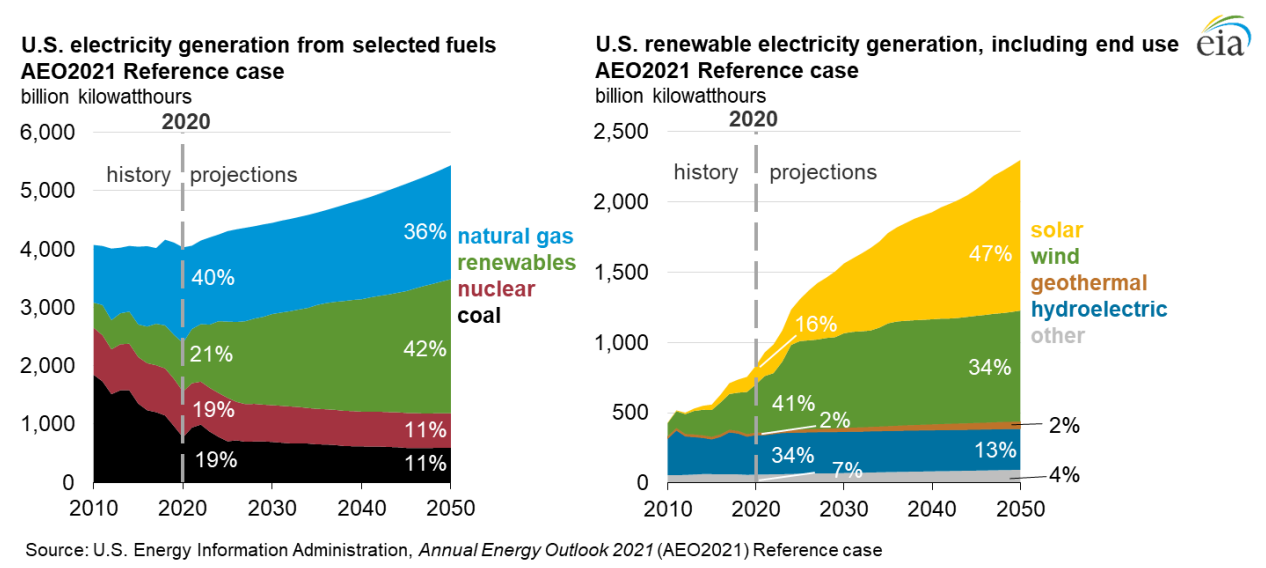
\includegraphics[scale=0.6]{Figure001-EIA_projections}
\caption[U.S. EIA projections based on the AEO2021 reference case]{U.S. EIA projections of (Left) U.S. electricity generation by sector and (Right) individual contributions by renewable type based on the AEO2021 reference case \protect\citep{us_energy_information_administration_annual_2021}}
\label{fig:eia_2021_projections}
\end{figure}

Lazard Asset Management breaks renewables down by \acrlong{lcoe} (\acrshort{lcoe}) in U.S. dollars/\acrshort{mwh}, where \acrshort{lcoe} is the estimated lifetime average net cost per unit energy of an electricity generating plant. In their 2020 analysis, intermittent energy sources like wind and utility-scale solar are already cost-competitive with fossil fuel-derived sources \citep{lazard_lazards_2020}. Geothermal, an “always on” source of power, ranges from \$59-\$101/\acrshort{mwh}  \acrshort{lcoe}, making it second-tier in cost competitiveness but comparable to community and rooftop solar installations \citep{lazard_lazards_2020}. Overall, the transition in energy sources away from fossil fuel dominance is in progress, and the demand for energy in support of population growth and country development will remain a driver over the next 30 years.

\section{Upstream Commercial Pressures}\label{ch1:upstream}
Businesses focused on \acrlong{ep} (\acrshort{ep}) of oil and gas face a growing list of pressures influencing future corporate strategy. On one hand, the increase in energy consumption predicted in the \acrshort{aeo} and \acrshort{ieo} make the case for steadily ramping up production to provide plentiful supply to meet global demand. However, geopolitical tensions, state-ownership of oil companies, and breakthrough technologies create a volatile landscape unforgiving of an unsophisticated production approach. In just the past 15 years, major downturns in oil prices were triggered by a mixture of factors: the financial crisis tied to banking practices and housing market instability in 2008 \citep{singh_2007-2008_2021}, increased production from U.S. unconventional plays and supply decisions from the \acrlong{opec} (\acrshort{opec}) in 2014 \citep{lioudis_what_2021}, and a price war between Russia and Saudi Arabia coinciding with a global pandemic in 2020 \citep{blessing_what_2021}. Additional uncertainty comes from national oil companies that control the majority of the world’s petroleum reserves, production, and rights for exploration and development. These state-run enterprises can eschew free market principles, favoring national priorities over efficient operations, oil field sustainability, business transparency, and maximizing shareholder value \citep{pirog_role_2007}. Meanwhile, disruptive technologies like precise directional drilling and hydrofracturing have provided access to previously cost-prohibitive reserves, changing the balance of power as countries like the U.S. and China become less reliant on foreign hydrocarbon imports \citep{shuen_dynamic_2014}.

Layered on top of these strategic influences are the unexpected events that have enormous influence over energy production and distribution operations. The 2020 outbreak of the COVID-19 virus acted as an accelerator on longer-term trends of digital transformation and decarbonization in the oil \& gas industry. In the wake of a 25\% decrease in global demand, companies responded with massive layoffs and restructuring, a heightened focus on digitalization, and portfolio rationalizations that include shale write-downs and asset divestments \citep{deloitte_2021_2020}. Extreme weather events are presenting reflective moments on how energy is managed now and in the future. Winter storm Uri blanketed Texas in record low temperatures in February 2021, shutting down liquid fuel supply and electricity generation from natural gas, coal, nuclear, and wind-based power plants, with downstream power blackouts, water outages, and surge pricing on electricity that impacted millions \citep{harc_winter_2021,lazard_lazards_2020}. And additional threats loom in the cyberworld as malicious hacking activities have rippling social and financial implications. One such attack on Colonial Pipeline, which handles almost 50\% of the liquid fuels supplied to the U.S. East Coast, led to gasoline shortages, price spikes, chemical factory shut-downs, and worldwide news coverage until the hefty ransom was paid in May 2021 \citep{sanger_pipeline_2021}.

\section{Net Zero Ambitions}\label{ch1:netzero}
The 2015 Paris climate agreement set a target of <2℃ on the rise in global temperatures above the pre-industrial average (i.e., the period from 1850-1900) to prevent the most extreme modeled impacts of climate change \citep{unfccc_paris_2015}. The more commonly-ascribed 1.5℃ target may be unachievable given current trajectories, and international calls to action focus on reducing anthropogenic carbon dioxide emissions to “net zero” as quickly as possible \citep{ipcc_global_2018}. Greater public awareness and discussion about these target puts pressure on the energy industry to redefine their traditional business models. Beginning in 2020, top-tier oil and gas companies started issuing press releases outlining energy transition targets for 2025, 2030, 2050, and beyond \citep{bp_international_2020,chevron_chevron_2021,conocophillips_conocophillips_2020,equinor_equinor_2020,exxonmobil_exxonmobil_2021,shell_responsible_2020,shell_shell_2021,total_total_2020,total_2020_2021}. The proposed strategies vary but generally focus on (i) reducing company stake in fossil fuel exploration and production activities, (ii) setting a net zero target applicable to emissions from operations, product carbon intensity, and carbon offsets, and (iii) dedicating investments in low and no-carbon energy alternatives to replace hydrocarbons. Nevertheless, pressure to do more, faster reached a new peak in May 2021; a court decision in The Netherlands and shareholder votes for two U.S. majors demanded an accelerated push toward emissions reductions and low-carbon energy options \citep{mcwilliams_investors_2021}.

\section{Geothermal Energy}\label{ch1:geothermal}

\section{Research Questions}\label{ch1:researchqs}
